% ===================== PARTE 8: MEMORIA RETENIDA (nueva) =====================
\parte{Memoria retenida}{Memoria retenida: ¿quién deja basura?}
  {Liberar en el acto es la promesa del paper. Se contó, instante a instante, cuántos bloques de memoria deja vivos cada algoritmo.}{p8_portada}

\begin{frame}{Anderson guarda una caja de pendientes; los demás liberan en el acto}
  \fuente{herramientas/bench\_basura.cpp; docker y nativo\_oficial/basura.csv; EXPLICACION.md, Parte 6.3}
  \begin{columns}[T]
    \column{0.5\textwidth}
    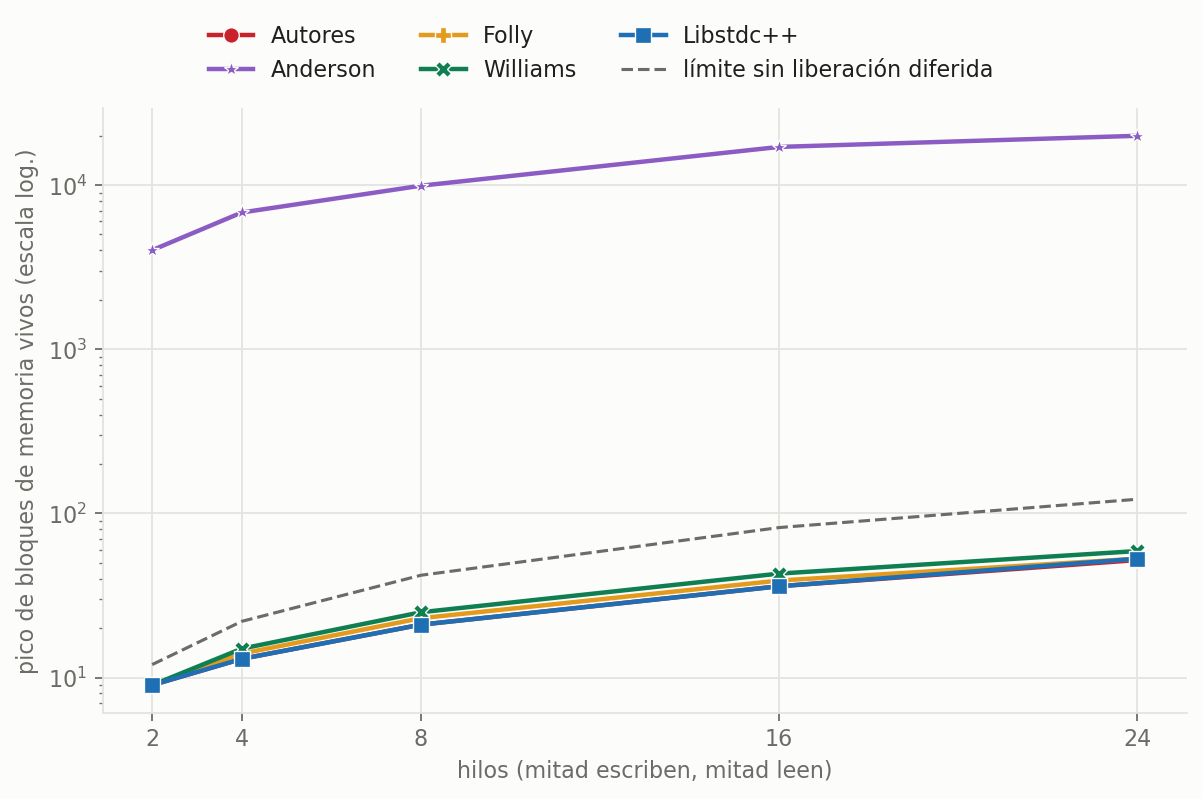
\includegraphics[width=\linewidth]{figuras/memoria_retenida}
    \column{0.46\textwidth}\footnotesize\renewcommand{\arraystretch}{1.12}
    \begin{tabular}{@{}rrrrr@{}}
      \toprule
      \textbf{Hilos} & \textbf{Límite} & \textbf{Autores} & \textbf{Anderson} & \textbf{Otros}\\
      \midrule
      2 & 12 & 9 & \textbf{4\,013} & 9\\
      8 & 42 & 21 & \textbf{9\,910} & 21-25\\
      24 & 122 & 52 & \textbf{19\,960} & 53-59\\
      \bottomrule
    \end{tabular}
    \par\smallskip\scriptsize Pico de bloques vivos; la mitad de los hilos escribe y la otra mitad lee. «Límite»: el máximo si todo se liberara en el acto (fórmula del equipo, no del paper).
    \par\medskip
    \caja{Cuatro líneas casi pegadas, siempre bajo el límite. Anderson, con 24 hilos, unas \textbf{380 veces más bloques}.}
  \end{columns}
  \nota{p8_memoria}
\end{frame}

\begin{frame}{Antes de condenar a Anderson: tres matices}
  \fuente{docker y nativo\_oficial/basura.csv; tablas.md, «Memoria retenida»; EXPLICACION.md, Parte 6.3}
  \begin{columns}[T]
    \column{0.6\textwidth}
    \begin{enumerate}\small\setlength{\itemsep}{6pt}
      \item \textbf{Solo espera el bloque de control.} El objeto muere en el acto: su pico de objetos vivos es 14, como los demás y bajo el límite de 37.
      \item \textbf{En bytes es poco.} 469\,KB frente a 2,3\,KB de Autores: 200 veces más, pero menos de medio mega.
      \item \textbf{La memoria total no lo delata.} Con $n = \pot{6}$ y 24 hilos, Anderson usa 910\,MB y Autores 1\,074\,MB: ahí pesan los datos.
    \end{enumerate}
    \column{0.36\textwidth}
    \caja{\textbf{Sin Docker, lo mismo:} Anderson llega a 20\,256 bloques (476\,KB); los demás, entre 53 y 59, bajo el límite de 122.}
    \par\medskip
    \caja{\textbf{Veredicto de la fila 13:} «Anderson tiene un pequeño sobrecoste; Autores, ninguno»: \sirep.}
  \end{columns}
  \vfill
  \porque{la caja de pendientes}{Anderson no libera un bloque mientras algún lector pueda estar usándolo: lo deja en una caja y la vacía cada 2\,000 retiradas, tras revisar los \emph{hazard pointers} de todos. Compra velocidad de lectura con esa caja. Autores no la necesita: el peso le dice en el acto que ya nadie lo usa.}
  \nota{p8_matices}
\end{frame}
